%%This is a very basic article template.
%%There is just one section and two subsections.
\documentclass{assign}

\usepackage[textwidth=4cm, textsize=footnotesize,
colorinlistoftodos, shadow]{todonotes}
\usepackage{textcomp,xspace}
\usepackage{varioref,dsfont}
\usepackage{setspace}

\newcommand{\R}{\ensuremath{\mathds{R}}}
\newcommand{\Q}{\ensuremath{\mathds{Q}}}
\newcommand{\N}{\ensuremath{\mathds{N}}}
\newcommand{\I}{\ensuremath{\mathds{I}}}
\newcommand{\E}{\ensuremath{\mathds{E}}}
\newcommand{\Z}{\ensuremath{\mathds{Z}}}
\newcommand{\D}{\ensuremath{\mathds{D}}}
\newcommand{\W}{\ensuremath{\mathds{W}}}
\newcommand{\B}{\ensuremath{\mathds{B}}}
\newcommand{\Sn}{\ensuremath{\mathds{S}}}

% Define a counter for the inserted todonotes.
\newcounter{todoListItems}
\newcommand{\todoTrans}[2][ ]{%
	% Increment counter
	\addtocounter{todoListItems}{1}%
	\todo[%
		caption={\protect\hypertarget{todo\thetodoListItems}{}#2},
		#1]
	{
		#2 \hfill
		\hyperlink{todo\thetodoListItems}{$\uparrow$}
	}
}

\newcommand{\addref}{\todoTrans[color=blue!40]{Needs reference.}\xspace}
\newcommand{\addcontent}[1]{\todoTrans[color=green!40, inline]{#1}\xspace}
\newcommand{\rewrite}[1]{\todoTrans[color=red!40]{#1}\xspace}
\newcommand{\clarify}[1]{\todoTrans[color=orange!40]{#1}\xspace}

\newcommand{\thetas}{\boldsymbol{\theta}}
\newcommand{\data}{\mathcal{D}}
\newcommand{\given}{\mid}

\mathchardef\ordinarycolon\mathcode`\:
\mathcode`\:=\string"8000
\begingroup \catcode`\:=\active
  \gdef:{\mathrel{\mathop\ordinarycolon}}
\endgroup


\title{Restricted Boltzmann Machines for Computer Vision}
\author{Tom Brosch}

\begin{document}
%\doublespacing

\listoftodos
\newpage
\maketitle
\tableofcontents
\newpage

\begin{abstract}
Learn image segmentation from unlabelled training data.
\end{abstract}

%------------------------------------------------------------------------------
%								INTRODUCTION
%------------------------------------------------------------------------------
\section{Introduction}

\subsection{Overview}

I will only state the basic results without any proof or derivation. References
are provided for further reading.

\subsection{The Basics}

\subsubsection{Machine Learning Terminology}

This section introduces the basic terminology that is used throughout the
proposal. Knowledge about a problem domain is modelled as a probability
distribution $p(\vect{x}\given \boldsymbol{\theta}, \mathcal{M})$, conditioned on
the probabilistic model $\mathcal{M}$ and its parameters
$\boldsymbol{\theta}$.
The probabilistic model $\mathcal{M}$ is chosen a priori based on prior
knowledge about the problem domain. The parameters $\boldsymbol{\theta}$ of the model are inferred from
training samples. This process of inferring the parameters of the model given
training examples is referred to as \emph{learning} or \emph{model fitting}. The
process of inferring the values of some components of the vector given other
components of the vector is referred to as \emph{prediction}.

The different components of the vector can be divided according to different
criteria.
\begin{description}
  \item[Visibility] All observed variables are referred to as visible units or
  just \emph{visibles}. The unobserved variables are referred to as hidden units
  or just \emph{hiddens}.
  \item[Role] Variables that act as input for a prediction task are referred to
  as input units or \emph{features}. The output variables are referred to as
  \emph{response variables}.
  \item[Interest] Hidden variables which are of interest are referred to as
  \emph{query variables}. The remaining variables are referred to as \emph{nuisance
  variables}.
\end{description}

Prediction is refined into classification and regression. If the response
variables take on discrete values, prediction is referred to as classification.
If the response variables are continues, prediction is referred to as
regression. Learning can also be divided into supervised and unsupervised
learning. Supervised learning when the inputs and outputs are part of the
training set. Unsupervised learning is when only the inputs and not the outputs
are part of the training set.

\subsubsection{Notation}

Vectors are small caps bold Latin letters. Models and sets are capital
calligraphic. Matrices are capital bold Latin letters.

Unless otherwise noted, inputs are x and outputs are y. Visibles are v and
hiddens are h. Model parameters in general are denoted as $\boldsymbol{\theta}$.
The variables $i, j, k$ are used as integers describing an index. $M$ number of
features. $N$ number of training examples. $\vect{X}$ is an $N$ by $M$ matrix
containing the training set. Samples are organized row-wise. Data set in set
notation $\mathcal{D}$. I use the hat to denote an estimate. For example
$\hat{\thetas}$ is an estimate of $\thetas$. An optional index indicates the
method that was used to estimate $\thetas$, e.g. $\hat{\thetas}_\text{Method}$.

$\vect{W}$, matrix. $w_{ij}$, $(i,j)^\text{th}$ element of $\vect{W}$.
$\vect{w}_{i, \cdot}$ row vector. $\vect{w}_{\cdot, j}$ column vector.
$x, y, z \in \R$. All indices are 1-based.

\subsubsection{Probability Terminology}

A probability $p(x)$ is a function of $x$ with the
following properties:
\begin{itemize}
  \item $p(x) \in [0, 1]$
  \item $\int_x p(x)\,dx = 1$ (continuous case)
  \item $\sum_x p(x) = 1$ (discrete case)
\end{itemize}

A \emph{generative model} $p(\data \given \thetas)$ is a function of $\data$
that assigns a probability to $\data$ that $\data$ has been generated by the
model.

The \emph{likelihood function} $L(\thetas)$, or just \emph{likelihood} for
short, is a function of $\thetas$ defined as $L(\thetas) = p(\data \given
\thetas)$. It describes to probability of the data $\data$ given the model and
model parameters $\thetas$\footnote{and not the probability of the parameters
$\thetas$ given the data.}. It is worth noting that the likelihood is not a
probability since $\int_{\thetas} L(\thetas)\,d\thetas \neq 1$ in general.

It is also possible to calculate the probability of $\thetas$ given $\data$
using Bayes' Theorem:
\begin{equation}
p(\thetas \given \data) = \frac{p(\data \given \thetas)p(\thetas)}{p(\data)}
\end{equation}
In this context, $p(\thetas \given \data)$ is called the posterior, $p(\data
\given \thetas)$ is called the likelihood, $p(\thetas)$ is called the prior, and
$p(\data)$ is called the evidence or marginal likelihood\footnote{It is called
marginal likelihood, because it can be obtained by marginalizing over the
parameter $\thetas$: $p(\data) = \int p(\data, \thetas)d\thetas = \int
p(\data\given\thetas)p(\thetas)d\theta$}.

\subsubsection{Introduction to Learning}

Learning means to infer the model parameters such that a measure of the fit of
the model and the data is optimized. If we chose the likelihood, $p(\data
\given \thetas)$, as the objective function, the method is called maximum
likelihood estimation (MLE).
\begin{align}
\hat{\thetas}_\text{MLE} &= \arg\max_{\thetas} L(\thetas)\\
\label{eq:mle}
\intertext{with}
L(\theta) &= p(\data \given \thetas)
\end{align}
In practice, the negative log likelihood, $-\log p(\data \given \theta)$, is often
minimized instead, which gives identical results as using \vref{eq:mle}.

You can also use the posterior as the objective function. The process of
maximizing the posterior distribution is known as \emph{maximum a posterior}
(MAP) estimation.
\begin{align}
\hat{\thetas}_\text{MAP} &= \arg\max_{\thetas} p(\thetas\given\data) \\
\intertext{Since the evidence does not depend on $\thetas$, it is sufficient to
maximize $p(\thetas\given\data) \propto p(\data\given\thetas)p(\thetas)$}
\hat{\thetas}_\text{MAP} &= \arg\max_{\thetas}p(\data \given \thetas)p(\thetas)
\end{align}

\subsubsection{Graphical Models}

Useful when defining the joint probability over a large set of variables.
Conditional independence can be expressed by mean of a graph. Each node
represents a random variable. The lack of an edge represents conditional
independence. If the graph forms an undirected acyclic graph (DAG) is is called
a directed graphical model (DGM). If all edges are undirected, it is called
an undirected graphics model (UGM).

The direction of edges in a DGM implies a topological order that can be used the
define the joint probability.
\begin{equation}
p(v_1, \dotsc, v_n) = p(v_1)p(v_2\given v_1)\dotsm p(v_n\given v_1, \dotsc
v_{n-1})
\end{equation}

An example of a DGM is the quick medical reference (QMR) network.
A bipartite graph was used to model the relationship between 570 diseases and
4075 symptoms (see \vref{fig:qmr}). Given the independency constraints from the
graph, the joint probability can be simplified to:
\begin{equation}
p(\vect{v}, \vect{h}) = \prod_s p(h_s) \prod_t p(v_t\given
\vect{h}_{\text{pa}(t)})
\end{equation}
where $\vect{h}_{\text{pa}(t)}$ denotes the vector of all parent nodes of node
$v_t$.

\begin{figure}
\centering
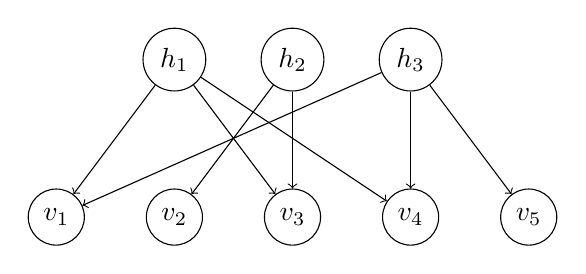
\begin{tikzpicture}
\tikzstyle{gnode}=[shape=circle,draw=black,font=\sffamily]

\foreach \x in {1,...,3} {
	\node[gnode] (h\x) at (1.5*\x + 1.5, 0) {$h_\x$};
}
\foreach \y in {1,...,5} {
	\node[gnode] (v\y) at (1.5*\y, -2) {$v_\y$};
}
\draw[->] (h1)--(v1);
\draw[->] (h1)--(v3);
\draw[->] (h1)--(v4);
\draw[->] (h2)--(v2);
\draw[->] (h2)--(v3);
\draw[->] (h3)--(v1);
\draw[->] (h3)--(v4);
\draw[->] (h3)--(v5);
\end{tikzpicture}
\caption{Quick medical reference (QMR) network with 3 diseases and 5
symptoms. A DAG is used to represent dependencies between symptoms and
diseases. The symptoms are the visible variables and the diseases are the
hidden causes which are to inferred given the symptoms.}
\label{fig:qmr}
\end{figure}

\subsection{Deep Belief Networks}

\subsubsection{Introduction}

Graphical models can be used to model the way humans are believed to perceive
their environment. There is evidence that the human brains tried to interpret
images be means of simple shaped. The example image\addcontent{Image which is
composed of simple shaped.} could be composed of 4 strange shapes. A more
natural explanation would be that the image is composed of a black square and a
white circle. Images are composed of basic shapes or image features. This idea
can be modelled using a graphical model. Speaking in the language of a graphical
model similar to the QMR, the pixels of an image are the observed variables or
visibles and the presence of a black square and a white circle are the hidden
variables that cause the pixel to take on the colors that they take
on.\addcontent{2 layer DGM for the previous case. 4 Shapes, lots of pixels.} If
we make the connections undirected we get a Restricted Boltzmann Machine (RBM).

\begin{figure}[tb]
\centering
\subfigure[Basic Shapes]{
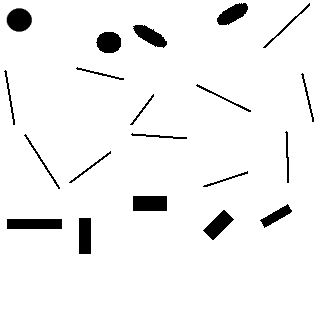
\includegraphics[width=0.2\textwidth]{images/features.png}
}
\subfigure[Test samples]{
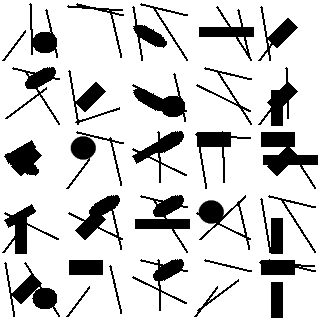
\includegraphics[width=0.2\textwidth]{images/testset.png}
}
\subfigure[RBM]{
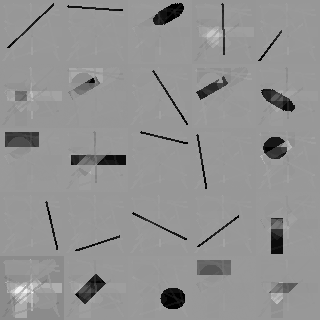
\includegraphics[width=0.2\textwidth]{images/rbm_32.png}
}
\subfigure[PCA]{
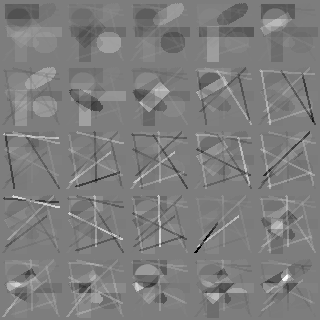
\includegraphics[width=0.2\textwidth]{images/pca.png}
}
\caption{The 20 basic shapes are shown in (a). These shapes were then combined
to form new images. 25 samples are shown in (b). An RBM and principle component
analysis (PCA) was used to extract features from the training set. Features
found by an RBM (c) correlate very strongly with the 20 basic shapes used to
build the training set. Features found by PCA (d) don't capture the true shapes
well.}
\label{fig:rbmotivation}
\end{figure}

When humans can learn to decompose an image into basic shapes, can an RBM learn
basic shapes as well? I have set up a small experiment to demonstrate the
learning capabilities of RBMs. Therefore, I have created 20 basic shapes---4
elliptic shapes, 5 rectangular shapes, and 11 strokes---with a resolution of $64
\times 64$ pixels. I have created a test set of 5000 images where each image was
composed of 3 to 4 randomly chosen shapes. I have then used an RBM to extract 25
features from the training set \footnote{$64 \times 64 = 4096$ visible units.
25 hidden units. 10000 epochs. Batch size 100. Learning rate 0.003. Sparsity
target 0.15. Sparsity penalty 0.1. Weight decay, momentum 0.9}.
Results are shown in figure ??. Figure ??d shows the first 25 features found by
principal component analysis. Without any prior knowledge about the shapes, the
RBM was able to learn the basic shapes the images were composed of just from the
training data. Neural network interpretation: Neurons fire specifically to the
presence of a shape. The network has learned to form circle neurons which are
active only if the image contains a circle. The experiment should serve as a
motivation that RBMs can be the building blocks of a more elaborate system that
can learn to segment images using unlabelled training data.\clarify{What do the
images actually show? The weights of the edges. The image that is created when
a given hidden unit is active. The receptive field of a hidden neuron. Basis
functions of the image. Even though the image is not a linear combination in
the binary case.}

%RBMs have been used to find structure in images. The features of
%hand-written digits are basic strokes.\addref The features of natural images
%are edge detectors.\addref

\begin{figure}[tb]
\centering
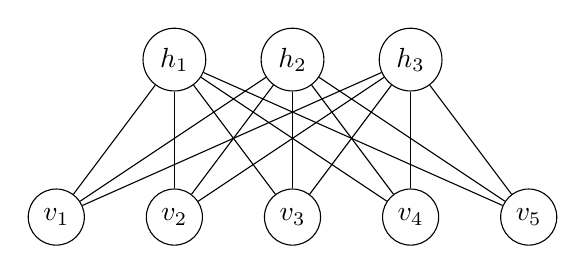
\begin{tikzpicture}
\tikzstyle{gnode}=[shape=circle,draw=black,font=\sffamily]

\foreach \x in {1,...,3} {
	\node[gnode] (h\x) at (1.5*\x + 1.5, 0) {$h_\x$};
}
\foreach \y in {1,...,5} {
	\node[gnode] (v\y) at (1.5*\y, -2) {$v_\y$};
}
\foreach \x in {1,...,3} {
	\foreach \y in {1,...,5} {
		\draw (h\x)--(v\y);
	}
}
\end{tikzpicture}
\caption{RBM with 5 visible and 3 hidden units.}
\label{fig:fig1}
\end{figure}

It is also natural to create hierarchies of image features. Images are composed
of basic image features, whereas a combination of image features themselves are
caused by higher level image features. E.g. the presence of several circles are
caused by the higher lever feature face. Hierarchies of features can be modelled
using deep architectures. A straight forward way to stack multiple layers of
features representations together is shown in figure ??a). Alternative are to
use a fully undirected deep model also unknown as Deep Boltzmann Machine (DBM)
or deep model consisting of mostly directed layers except for the first layer
which is an undirected layer. This model is called a Deep Belief Network (DBN).
A DBN can be composed by stacking together several RBMs. This makes learning and
inference efficient since both tasks can be performed in each layer.\rewrite{Bad
language.}

\subsubsection{Restricted Boltzmann Machines}

A Restricted Boltzmann Machine is an undirected graphical model. It consists of
two layers. There are no connections between variables in one layer. Variables
of different layers are fully connected. Furthermore, given one layer, variables
of the other layer are conditional independent. The bottom layer is often
referred to as the observed or visible variables. Variables of the top layer are
often referred to as the hidden variables. The joint probability is given by the
energy function.\clarify{Binary case.}

\begin{table}
\centering
\begin{tabular}{@{}>{$}c<{$}l@{}}
\toprule
\text{Symbol} & Description \\
\cmidrule(r){1-1} \cmidrule(l){2-2}
V					& $V \in \N$, Number of visible units\\
H \in \N			& Number of hidden units\\
N					& Number of samples \\
i					& Integer indexing the visible units \\
j					& Integer indexing the hidden units \\
n					& Integer indexing the samples \\
\vect{v}			& $V \times 1$ vector containing the visible units\\
\vect{h}			& $H \times 1$ vector containing the hidden units\\
\vect{W}			& $V \times H$ matrix containing the weights \\
w_{ij}				& Weight of the edge between $v_i$ and $h_j$ \\
\vect{w}_{i, \cdot}	& $i$th row vector of $\vect{W}$, i.e. $\vect{w}_{i,
\cdot} = [w_{i1} \dotso w_{iH}]^{T}$ \\
\vect{w}_{\cdot, j} & $j$th column vector of $\vect{W}$, i.e.
$\vect{w}_{\cdot,j} = [w_{1j} \dotso w_{Vj}]^{T}$\\
\vect{b}			& $V \times 1$ vector containing the visible biases \\
\vect{c}			& $H \times 1$ vector containing the hidden biases \\
\vect{V}			& $N \times V$ matrix containing the visibles in each row \\
\vect{H} 			& $N \times H$ matrix containing the hiddens in each row \\
\vect{B}			& $N \times V$ matrix containing the visible biases in each row\\
\vect{C} \in \R^{N \times H}			& Matrix containing the hidden
biases in each row\\
\bottomrule
\end{tabular}
\caption{Notation}
\label{tab:notation}
\end{table}

\begin{align}
p(\vect{v}, \vect{h} \given \boldsymbol{\theta}) &=
\frac{1}{Z(\boldsymbol{\theta})}e^{-E(\vect{v}, \vect{h} \given
\boldsymbol{\theta})} \\
\intertext{with}
-E(\vect{v}, \vect{h}\given \boldsymbol{\theta}) &= \sum_{i, j}v_i w_{ij} h_j +
\sum_i b_i v_i + \sum_j c_j h_j \\
&= \vect{v}^\textup{T}\vect{W}\vect{h} + \vect{b}^\textup{T}\vect{v} +
\vect{c}^\textup{T}\vect{h}
\end{align}
with $\vect{W} \in \R^{V \times H}$ and $\thetas = \{\vect{W}, \vect{b},
\vect{c}\}$.

The joint density of the visible units is given by (in the binary case)
\begin{align}
p(\vect{v} \given \thetas) &= \frac{1}{Z(\thetas)}\sum_{\vect{h}}e^{-E(\vect{v},
\vect{h} \given \thetas)} \\
&= \frac{1}{Z(\thetas)}e^{-F(\vect{v} \given \thetas)}\\
\intertext{with}
-F(\vect{v} \given \thetas) &= \vect{b}^\text{T}\vect{v} + \sum_{j = 1}^H \log(1
+ \exp(\vect{w}_{\cdot,j}^\text{T}\vect{v} + c_t))
\end{align}\clarify{Need a notation for column and row vector and component.}
In this context $F(\vect{v} \given \thetas)$ is called the free energy of the
RBM. The free energy plays an important role for supervised learning tasks like
classification.

\subsubsection{Inference}

Inference of the hiddens or the visibles can be done efficiently in an RBM. In
general:\clarify{$p(h_j \given \vect{v})$ is Bernoulli distributed.}

\begin{align}
p(h_j = 1 \given \vect{v}, \thetas) &= \sigm(\Delta E_j)\\
p(v_i = 1 \given \vect{h}, \thetas) &= \sigm(\Delta E_i)\\
\intertext{with $\sigm(x) = (1+e^{-x})^{-1}$ is the sigmoid function and}
\Delta E_j & := E(h_j = 0) - E(h_j = 1) \\
\Delta E_i & := E(v_i = 0) - E(v_i = 1) \\
\intertext{Plugging in the energy function of a binary RBM yields}
p(h_j = 1 \given \vect{v}, \thetas) &= \sigm(\vect{w}_{\cdot,j}^\text{T}\vect{v}
+ c_j)\\
p(v_i = 1 \given \vect{h}, \thetas) &= \sigm(\vect{w}_{i,
\cdot}^\text{T}\vect{h} + b_i)
\end{align}
Since the visibles are conditional independent given the hiddens and vice versa,
one can calculate $\E[\vect{h} \given \vect{v}, \thetas]$ and $\E[\vect{v}
\given \vect{h}, \thetas]$ in parallel for each training sample using
\begin{align}
\label{eq:hgivenv}
\E[\vect{h} \given \vect{v}, \thetas] &= \sigm(\vect{W}^\text{T}\vect{v} +
\vect{c})\\
\label{eq:vgivenh}
\E[\vect{v} \given \vect{h}, \thetas] &= \sigm(\vect{W}\vect{h} + \vect{b})\\
\intertext{and multiple samples from the training set using}
\E[\vect{H} \given \vect{V}, \thetas] &= \sigm(\vect{V}\vect{W} +
\vect{C})\\
\E[\vect{V} \given \vect{H}, \thetas] &= \sigm(\vect{H}\vect{W}^\text{T} +
\vect{B})
\end{align}

\subsubsection{Sampling}

You can sample the conditionals easily using \vref{eq:hgivenv} and
\vref{eq:vgivenh}, respectively. Recall that the visibles and hiddens are
Bernoulli distributed. Hence:
\begin{align}
\text{Ber}(x \given \theta) &= \theta^{\I(x = 1)}(1-\theta)^{\I(x = 0)} \\
\E[\text{Ber}(x \given \theta)] &= \theta
\end{align}
Therefore, one can sample $\vect{v} \sim p(\vect{v} \given \vect{h})$ and
$\vect{h} \sim p(\vect{h} \given \vect{v})$ using
\begin{align}
\vect{v} &= \I(\vect{x} < \E[\vect{v} \given \vect{h}]) & \text{with $x_i \sim
\text{U}(0,1)$}\\
\vect{h} &= \I(\vect{y} < \E[\vect{h} \given \vect{v}]) & \text{with $y_j \sim
\text{U}(0,1)$}
\end{align}

Getting a sample from the joint directly is not possible. One can sample from
$p(\vect{v}, \vect{h} | \thetas)$ using Block Gibbs sampling. Initialize
$\vect{v}$ with random values. Then, sample from $p(\vect{h} \given \vect{v})$
and $p(\vect{v} \given \vect{h})$ alternately. Do this until the burn-in. Now
you can draw samples from the joint. This can take quite long.

\subsubsection{Learning}

\addcontent{Learning rules. Learning tricks: Weight decay, momentum,
mini-batches, GPU implementation.}

General learning rule. Then, how to approximate the components. One with mean
field approximation. The other one with Monte Carlo approach. Sample from the
model can calculate expectation. Algorithms differ in how to sample from the
model. Stochastic gradient descent. Just name it and reference according papers.
More popular is contrastive divergence. Set visibles to the data sample and do
one block Gibbs sampling operation. Write basic equations.

Tricks to get it work. Weight decay, momentum, mini-batches. Write down
algorithm in psydo code.

Comment on GPU implementation. Basicely matrix operations that can be calculated
in parallel using cublas.

\subsubsection{Sparse Coding}

Penalty term from Ng and Hinton.

\subsubsection{Non-binary Restricted Boltzmann Machines}

\addcontent{Gaussian-Bernoulli RBMs}
\addcontent{Rectangular Units}

\subsection{Training of Deep Belief Networks}

Problems of deep belief networks: Explaining away. Hard to train. Introduce
complementary priors. DBN with complementary priors is equal to RBM. Train a DBN
by greedy layer-wise training of RBMs. Find tuning of weights of a DBN possible
but often not necessary in practice.

\subsection{Applications}

\subsubsection{Generating Images}

\addcontent{Use an RBM to generate natural images (Hinton), Semi-RBM (cite
paper), Images of the CC (own work), Segmentations of the CC (own work)}

\subsubsection{DBN for Learning of Image Features}

Of hand-written digits. Learning of edge detectors. Basic strokes with sparsity
target.

\subsubsection{DBNs for Classification}

Combined supervised and unsupervised learning task. Features are learned
unsupervised. Labels are learned supervised. Labels are used to label the
classes that could be found in an unsupervised manner. Classification using free
Energy or clamped block Gibbs sampling.

\addcontent{Claim: Need only a few labels to get good classification results!
(Full testset for feature learning. Only a few labelled cases to learn the
highest level.)}
\addcontent{Claim: Unlabelled data improves the results. (Train features only
with data, for which I have labels. Compare to when I use all data to learn
features.)}

\subsection{Different Flavours of RBMs}

\subsubsection{Convolutional RBMs}

Learning hierarchical models. Invariant to small translation.

\subsubsection{Gated RBMs}

Original work. Factored gates RBMs. Used to learn transformation with random dot
images.

%------------------------------------------------------------------------------
%							WORK ACCOMPLISHED
%------------------------------------------------------------------------------
\section{Work Accomplished}

\subsection{Generative Hierarchical Models for Image Representation}

My convolutional approach. Generalization. Specificity.

\subsection{Segmentation as a Regression Problem}

Is it classification or regression. I would say it is discrete regression but
not categorical. RBM for segmentation of the corpus callosum. Preliminary
results.

%------------------------------------------------------------------------------
%							   FUTURE WORK
%------------------------------------------------------------------------------
\section{Future Work}

\subsection{Unsupervised Learning of Models of Shape and Appearance}

\appendix

\section{Ideas for the Presentation}

Draw RBM with big circles and thin lines. Redraw it with over big lines and
small circles. Key are the lines and not the circles. Lines are the weights. The
weights determine the RBM.

\end{document}
